\documentclass[10pt,letterpaper]{article}
\usepackage[margin=1in]{geometry}
\usepackage{amsmath,amssymb,array,graphicx,url}
\usepackage{fancyhdr}
\setlength{\emergencystretch}{2em}
\setlength{\parskip}{2pt}
\setlength{\tabcolsep}{4pt}
\renewcommand{\arraystretch}{1.13}
\newcolumntype{L}[1]{>{\raggedright\arraybackslash}p{#1}}
\newcommand{\code}[1]{\texttt{#1}}
% Generated by scripts/render_results.py from measured data.
\newcommand{\OnlineRuns}{600}
\newcommand{\LoopInstances}{300,000}
\newcommand{\CorrectRuns}{600}
\newcommand{\ReferenceRuns}{432}
\newcommand{\MeasuredSeconds}{796.9}
\newcommand{\AbstractFinding}{Full-portfolio warm LinUCB achieves a paired geometric mean speed ratio of 1.011 (95\% CI 0.954--1.057) against native Q-learning and 1.002 (95\% CI 0.959--1.042) against exhaustive search, where ratios above one favor LinUCB. Against the training-selected fixed scheduler its ratio is 0.989 (95\% CI 0.932--1.031). The primary confidence intervals include one, so this campaign does not demonstrate a warm-start advantage. }
\newcommand{\MainResultsDiscussion}{Against Native Q-learning, warm LinUCB's paired geometric speed ratio is 1.011 (95\% CI 0.954--1.057); it is faster on 5 of the six input configurations. The interval crosses one, leaving the direction unresolved at this precision.

Against Exhaustive, warm LinUCB's paired geometric speed ratio is 1.002 (95\% CI 0.959--1.042); it is faster on 4 of the six input configurations. The interval crosses one, leaving the direction unresolved at this precision.

Against Best fixed, warm LinUCB's paired geometric speed ratio is 0.989 (95\% CI 0.932--1.031); it is faster on 4 of the six input configurations. The interval crosses one, leaving the direction unresolved at this precision.

None of the six warm-selector comparisons reaches a Holm-adjusted $p<0.05$ with six input-level signed-rank observations. Accordingly, the reported ratios and intervals are descriptive effect estimates.}
\newcommand{\ExplorationDiscussion}{At 50 instances the warm/native-Q speed ratio is 1.025 (95\% CI 0.980--1.083); at 144 it is 1.045 (95\% CI 0.999--1.106). At 500 instances, warm versus cold LinUCB gives 0.992 (95\% CI 0.949--1.024), while warm versus the context-free UCB baseline gives 1.006 (95\% CI 0.958--1.045). These prefix results share the same runs. They quantify exploration cost without counting prefixes as additional independent experiments.}
\newcommand{\ReductionDiscussion}{The reduced selector's 500-instance ratio against native Q-learning is 0.996 (95\% CI 0.962--1.032), and against exhaustive search it is 0.987 (95\% CI 0.949--1.030). Portfolio reduction therefore must be judged by measured runtime rather than by the nominal reduction from 12 to six arms.}
\newcommand{\OverheadDiscussion}{The median per-run median decision-plus-update cost is 1.60 microseconds for full warm LinUCB, 1.43 for the reduced selector, and 0.91 for exhaustive search. These costs are included in the reported runtime. Native Q-learning's main selection cost is inside the runtime and is included in loop time, so its external decision counter is not a comparable measure of algorithm overhead.}
\newcommand{\PracticalDiscussion}{Warm versus prior-only greedy selection has a paired ratio of 0.998 (95\% CI 0.963--1.022). The interval crosses one, leaving the direction unresolved at this precision. This control prevents attributing every gain from offline knowledge to online exploration. The median coefficient of variation of total time across the five runs of a scenario/selector is 5.0\%. This variability should be considered when interpreting percentage-level differences.}
\newcommand{\ConclusionFinding}{Measured warm/native-Q, warm/exhaustive, and warm/best-fixed speed ratios are 1.011, 1.002, and 0.989, respectively, on this environment. Their intervals include one: the expected warm-start improvement is not established. These outcomes describe a specific finite-horizon trade-off; they do not establish a universal winner.}
\newcommand{\PriorWeight}{0.25}
\newcommand{\RidgeValue}{1.0}
\newcommand{\AlphaValue}{0.025}
\newcommand{\ReducedArms}{STATIC, AutoLLVM, GSS, mFAC2, StaticSteal, AWFB}
\newcommand{\BestFixedArm}{AWFD}
\newcommand{\WallGap}{0.05}
\newcommand{\TransferRuns}{108}
\newcommand{\TransferInstances}{54,000}
\newcommand{\TransferDiscussion}{Against Best fixed, the exploratory warm-selector ratio is 0.984 (95\% CI 0.938--1.018). Against Prior greedy, the exploratory warm-selector ratio is 0.996 (95\% CI 0.978--1.016).}
\newcommand{\InterruptionSensitivity}{Native Q-learning: 1.017 (95\% CI 0.993--1.044); Exhaustive: 1.008 (95\% CI 0.973--1.047); Best fixed: 1.000 (95\% CI 0.966--1.035)}
\newcommand{\SelectionDiscussion}{Warm LinUCB tries a median of 11 distinct arms over 500 instances, versus 12 for cold LinUCB and 12 for context-free UCB. Its median modal-arm fraction is 93.2\%. These counts describe action concentration, not convergence to the best scheduler; using fewer arms is useful only if it reduces measured cost.}

\pagestyle{fancy}\fancyhf{}
\fancyhead[L]{\small Warm-Started Contextual Bandits for OpenMP Scheduling}
\fancyfoot[C]{\thepage}
\renewcommand{\headrulewidth}{0pt}
\title{\textbf{Warm-Started Contextual Bandits for OpenMP Scheduling:\\
A Reproducible Single-Node Study}}
\author{Shaan Chopra\quad Mrinal Dhami\quad Aniket Verma\\[3pt]
School of Computer Science and Engineering\\
Manipal Institute of Technology\\[3pt]
\small Group 3: 240905140\quad 240905026\quad 240905156}
\date{}
\begin{document}
\maketitle
\begin{abstract}
Choosing a loop scheduler online requires balancing scheduling quality against
the execution cost of discovering a good policy. We study whether offline
measurements and a small contextual bandit can reduce this cost in LB4OMP. A
native C++ harness selects among the same 12 scheduling algorithms available
to the released reinforcement-learning selector. Disjoint LinUCB models are
initialized from independent training inputs and compared with cold LinUCB,
context-free UCB, prior-only greedy selection, exhaustive search, the released
Q-learning implementation, and fixed schedules. The evaluation contains
\OnlineRuns{} online process runs and \LoopInstances{} measured loop instances
across 12 held-out scenarios, three workload families, and two thread counts
on a four-core Ryzen processor under WSL2. \AbstractFinding{}
All timings, output checks, training and validation configuration, dependency
patches, and analysis scripts are included in a reproducible artifact. The
results establish the behavior of this implementation on a modest multicore
system; they do not establish architecture-independent superiority or a new
bandit algorithm.
\end{abstract}
\noindent\textbf{Keywords:} OpenMP; scheduling algorithm selection; LB4OMP;
contextual bandits; warm start; empirical systems evaluation.

\section{Introduction}

The execution time of a parallel loop depends on how iterations are assigned
to threads. Static assignment has little dispatch overhead but may leave
workers idle when iteration costs vary. Dynamic assignment can improve balance
while increasing synchronization costs and disturbing locality. The OpenMP
schedule interface exposes this trade-off, and extended runtimes offer a wider
portfolio of scheduling techniques \cite{openmp,lb4omp}. Selecting a member of
this portfolio is an instance of the algorithm selection problem
\cite{rice}: the useful output is a fast algorithm for the current input and
machine, rather than an intrinsically best scheduler.

Online selection has an additional cost. Every trial consumes useful execution
time, including trials of algorithms that turn out to be poor. M\"uller
Kornd\"orfer et al. evaluate expert and reinforcement-learning selectors in
OpenMP and show that exploration can be expensive \cite{comparative}. Their
12-by-12 explore-first setup motivates a specific question: can prior
measurements reduce the cost paid before online selection becomes useful?

We implement an answer using warm-started disjoint LinUCB. The method observes
loop size, thread count, and an initial STATIC timing/imbalance probe, then
selects a scheduler for each execution of that loop. Offline ridge statistics
from separate inputs initialize the models. Training-only portfolio reduction
is evaluated separately. Both are existing ideas in algorithm selection and
bandit learning; the contribution here is their concrete, audited evaluation
in a public OpenMP runtime.

Our study asks three questions. \textbf{RQ1:} Does a warm-started selector
reduce measured execution cost relative to the released Q-learning selector?
\textbf{RQ2:} Does it improve on stronger practical alternatives, particularly
exhaustive search, a training-selected fixed arm, and prior-only selection?
\textbf{RQ3:} What changes when warm starting or portfolio reduction is removed,
and how large is the native selection overhead?

We provide three contributions: (1) an executable C++ evaluation using all 12
reference-portfolio schedulers; (2) a fixed training/test split with serialized
validation choices and unmodified scheduling logic; and (3) a measured
comparison that includes simple alternatives and confidence intervals at input
configuration level. The complete artifact accompanies this manuscript.

\section{Background and Related Work}

\subsection{Loop scheduling and automated selection}

LB4OMP extends LLVM's OpenMP runtime with dynamic and adaptive scheduling
methods \cite{lb4omp}. Auto4OMP adds expert selection and automatic chunk
calculation \cite{auto4omp}. These approaches address both the choice of a
scheduler and the granularity at which it dispatches work. Our implementation
uses the runtime's existing schedulers and expert chunk calculation directly;
it introduces no new chunk-generation algorithm.

The comparative study \cite{comparative} evaluates six applications on three
systems and compares expert selectors with Q-learning and SARSA. Its published
explore-first policy considers 144 ordered state--action combinations in a
12-algorithm portfolio. That budget corresponds to 28.8\% of a 500-instance
execution. The authors find that loop-time rewards are generally more useful
than imbalance alone and identify expensive exploration as a practical
limitation. We test the released Q-learning implementation on a smaller
machine and compare a contextual alternative against simple selectors.
Different hardware, inputs, compiler, and measurement boundaries mean this is
not a numerical replication of the published cluster results.

\subsection{Contextual bandits and warm starting}

UCB methods allocate trials using estimates and uncertainty
\cite{auer}. LinUCB models action rewards as linear functions of observed
context and uses a confidence term for exploration \cite{linucb}. Warm-start
bandits initialize these estimates with earlier knowledge. Oetomo et al.
study this problem theoretically and empirically, including the effects of
misspecified priors \cite{oetomo}. Consequently, initializing LinUCB from
offline data is not itself a novel learning algorithm. Our question concerns
the size and source of the resulting benefit in OpenMP scheduling.

STREAM and GAP motivate the regular streaming and graph workload families
\cite{stream,gap}. We use original compact kernels rather than claiming to run
either suite's reference implementation. Our uncertainty reporting follows the
systems-benchmarking principle that repeated loop samples must not be treated
as independent experimental replications \cite{kalibera}.

\section{Problem and Selection Method}

Let $\mathcal{A}=\{0,\ldots,11\}$ be the scheduling portfolio. At loop instance
$t$, an online selector chooses $a_t$ and observes the elapsed time
$T_t(a_t)$. The measured objective over horizon $H$ is
\begin{equation}
 C_H=\sum_{t=1}^{H}\left[T_t(a_t)+d_t+u_t\right],
 \label{eq:cost}
\end{equation}
where $d_t$ and $u_t$ are selector decision and update times outside the
parallel region. Native Q-learning's dispatch and learning execute inside
$T_t$, so they are already charged. Process startup, graph construction, and
final correctness checks are outside $C_H$, because the optimization target is
repeated loop execution. Wall-clock time around the complete online sequence
is logged separately to check the accounting.

\subsection{Context and reward}

Every external selector first executes one STATIC probe. Its context is
\begin{equation}
 x=\left[1,\log_2N,\log_2P,\log_2T_{\mathrm{probe}},
             L_{\mathrm{probe}},V_{\mathrm{probe}}\right]^\top.
\end{equation}
Here $L=1-\bar f/\max_p f_p$ is imbalance and
$V=\operatorname{std}(f_p)/\bar f$ is the coefficient of variation of thread
finish times relative to parallel-region start. These measures include thread
launch and arrival effects; they are not isolated per-iteration compute times.
The five non-intercept features are standardized using training-input
statistics, with a minimum scale of $10^{-8}$. No application identifier or test
ranking is supplied to the selector. The context remains fixed during a run;
adaptation comes from observed rewards, not from future information.

The scalar reward is
\begin{equation}
 r_t=\operatorname{clip}\left(
 -\frac{\log(T_t/T_{\mathrm{probe}})}{\log4},-1,1\right).
 \label{eq:reward}
\end{equation}
The probe time is fixed for that run. A fourfold slowdown maps to $-1$, while
a fourfold speedup maps to $1$. This bounded log-time reward stabilizes
learning but is a surrogate: maximizing expected clipped log reward need not
minimize expected arithmetic execution time under heavy tails. We therefore
evaluate Eq.~\ref{eq:cost}, and never substitute reward improvement for a
measured speedup.

\subsection{Warm-started disjoint LinUCB}

For each arm $a$, we retain independent ridge statistics
\begin{equation}
 A_a=\lambda I+w\sum_{i\in\mathcal{D}_{\mathrm{train}}}x_ix_i^\top,
 \qquad b_a=w\sum_{i\in\mathcal{D}_{\mathrm{train}}}x_i r_{i,a}.
 \label{eq:init}
\end{equation}
One median label per training scenario and arm is used, rather than counting
every correlated loop sample as separate prior evidence. The arm's estimate
is $\hat\theta_a=A_a^{-1}b_a$, and selection uses
\begin{equation}
 a_t=\arg\max_{a\in\mathcal{A}}
 \left[x^\top\hat\theta_a+\alpha\sqrt{x^\top A_a^{-1}x}\right].
 \label{eq:ucb}
\end{equation}
After a selected arm completes, $A_{a_t}$ gains $xx^\top$ and $b_{a_t}$ gains
$r_tx$. A Sherman--Morrison rank-one update maintains the inverse. With six
features and 12 arms, the inverse matrices and reward vectors occupy 4,032
bytes in double precision, excluding small metadata and the reduced-arm list.
The implementation observes only the selected action's online reward.

Cold LinUCB starts from $A_a=I$, $b_a=0$, while retaining the same training
scaler and exploration coefficient. It tests removal of all fitted prior
information, including prior regularization. Prior-greedy selection uses the
warm fitted model with $\alpha=0$ and no online update; it isolates what can
already be obtained through offline prediction.

\subsection{Portfolio reduction and chunk size}

The full portfolio is STATIC, SS, TSS, AutoLLVM, GSS, mFAC2, Static Steal,
AWF-B, AWF-C, AWF-D, AWF-E, and mAF. The reduced selector retains STATIC and
GSS as anchors. The other ten arms are clustered into four groups by average
linkage on training log-slowdown vectors. The medoid of each cluster is
retained, yielding six arms. Test data are excluded from clustering.
The selected representatives are \ReducedArms{}.

The primary experiment enables LB4OMP's existing expert chunk rule uniformly
for all selectors. In the pinned implementation this is
\begin{equation}
 m=\left\lfloor0.618\log_2\lfloor N/P\rfloor\right\rfloor,
 \qquad c=\left\lfloor\frac{N}{(2\cdot2^m)P}\right\rfloor.
\end{equation}
Our inputs keep $c\geq1$. Crucially, this rule also overrides STATIC's initial
chunk setting: the STATIC control uses cyclic chunks of size $c$, not a
single contiguous block per thread. That distinction limits comparison with
the common contiguous-static interpretation and can materially change
irregular-workload balance. We document it explicitly.

\section{Implementation and Experimental Design}

\subsection{Runtime and hardware}

Experiments execute on an AMD Ryzen 5 7235HS with four physical cores, eight
logical CPUs, and approximately 7.6\,GiB visible RAM, running Linux
\code{6.6.87.2-microsoft-standard-WSL2}. The compiler is Clang 16.0.6 with
\code{-O3 -std=c++17 -fopenmp -ffp-contract=off}. LB4OMP is pinned to commit
\code{b9d25eca7265a4b5b3a675a1765d489775847938}.
A portability patch replaces one initialized variable-length array with
\code{std::vector} and adds its header; scheduling and learning logic remain
unchanged. The runtime is built with OMPT enabled and x86 high-resolution
timer support. The artifact includes exact build commands and the patch.

Two and four threads are pinned to physical-core representatives
$\{0\},\{2\},\{4\},\{6\}$ with close binding. Dynamic teams are disabled.
The wait policy is active and the runtime block time is 200\,ms. The
\code{KMP\_CPU\_SPEED} value is 3200\,MHz for LB4OMP's internal tick conversion;
our external elapsed-time measurements use a monotonic clock independently.
Host power policy, turbo, temperature, and competing Windows activity are
uncontrolled. All conclusions are conditional on this WSL2 environment.

\subsection{Workloads and data split}

Table~\ref{tab:inputs} gives every input. A scenario is one workload,
configuration, and thread count. The two thread settings of each configuration
share an input identity and stay together in validation and bootstrap
resampling. Configurations 0 and 1 form training; 2 and 3 form testing. Thus
there are 12 training and 12 test scenarios, but only six independent test
input configurations.

\begin{table}[ht]
\centering\small
\caption{Input configurations. Each is measured at $P\in\{2,4\}$.}
\label{tab:inputs}
\begin{tabular}{lrrrr}
\hline
 & Train 0 & Train 1 & Test 2 & Test 3\\
\hline
Mandelbrot pixels & 16,384 & 65,536 & 25,600 & 50,176\\
Maximum pixel iterations & 96 & 120 & 144 & 168\\
Triad elements & 262,144 & 1,048,576 & 393,216 & 786,432\\
Triangle graph vertices & 512 & 2,048 & 1,024 & 1,536\\
\hline
\end{tabular}
\end{table}

Mandelbrot evaluates a square pixel grid with real coordinates
$[-2+s,1+s)$ and imaginary coordinates $[-1.2,1.2)$, where
$s=0.025(\mathrm{configuration}\bmod4)$. Escape iterations stop at radius two
or the configured iteration limit. The row-wise loop ordering produces
unequal work per pixel.

Triad computes $a_i=b_i+3c_i$ on double arrays initialized deterministically.
It represents regular streaming work. Its test working sets are approximately
9 and 18\,MiB across the three arrays; the smaller inputs may have substantial
cache reuse. We therefore call this a Triad-style kernel and do not claim
reference STREAM bandwidth results.

Triangle counting constructs an undirected graph with $24N$ proposed edges
using \code{std::mt19937} seeded with $1907+\mathrm{configuration}$. One third
of proposals have a hub-biased endpoint in the first $N/32$ vertices; the
others use uniform endpoints. Self-edges and duplicates are removed. Each
edge is oriented by vertex ID, and sorted neighbor-list intersections count
each triangle once. Construction is outside the timed loop. The graphs are
synthetic and cache-resident; this is not a measurement of GAP's reference
triangle-count implementation on large real-world graphs.

Each scenario repeats the same input for 500 instances. This primary study
evaluates stationary repeated loops. Phase-changing Mandelbrot, multi-socket
systems, and hardware-counter features were suggested in the synopsis but
are outside the implemented experiment. A separate exploratory test removes
one workload family from prior fitting.

\subsection{Training and protocol freeze}

Training calibration uses all 12 schedulers, three independent processes per
scenario/arm, and 20 logged loop instances per process. Each process performs
two untimed STATIC warm-ups, then one common timed STATIC probe and 19
instances of the requested fixed arm. Median runtime labels exclude the
probe; context features are the median of the 36 probe observations in a
scenario. The model uses these aggregate labels only.

We validate the grid $w\in\{0.25,1,4\}$,
$\lambda\in\{0.1,1\}$, and $\alpha\in\{0.025,0.1,0.4\}$ by leaving out one
workload/configuration group, including both thread counts, from the training
set. Scalers and ridge models are refitted in every fold. A deterministic
200-round simulation using measured training-fold median costs scores each
combination. This simulation selects hyperparameters; it is not counted as
measured online performance. The chosen values are
$w=\PriorWeight$, $\lambda=\RidgeValue$, and $\alpha=\AlphaValue$.
The best fixed training arm is \BestFixedArm{}, selected by geometric mean
runtime relative to training STATIC. Protocol and model files are written
before any final test measurement.

\subsection{Online baselines and timing}

We compare ten selectors (Table~\ref{tab:methods}). Every process uses the same
two warm-ups. Every external selector receives one timed STATIC probe; the
native Q-learning path starts with the upstream selector's STATIC
initialization. All 500 observations, including probes and exploratory
instances, are charged.

The warm selector is the primary tuned method. Cold LinUCB shares its
exploration coefficient, and context-free UCB uses a fixed coefficient of
0.1. These are diagnostic baselines, not independently optimized competitors.
The untuned exhaustive, fixed-arm, and prior-greedy controls are therefore
central to the practical interpretation.

\begin{table}[ht]
\centering\small
\caption{Compared selectors. Fixed choices use training information only.}
\label{tab:methods}
\begin{tabular}{L{2.7cm}L{11.9cm}}
\hline
Selector & Decision rule\\
\hline
STATIC / GSS & Fixed scheduler after the initial probe.\\
Best fixed & One training-selected arm, unchanged during test execution.\\
Exhaustive & One trial per arm over the first 12 instances; retain the lowest
observed time. No restart in stationary runs.\\
Native Q-learning & Released LB4OMP \code{auto,8}, zero table,
explore-first policy, learning and discount factors 0.5; reward constants
$(0.01,-2,-4)$ and post-exploration alpha decay 0.05.\\
UCB & Context-free reward mean plus
$0.1\sqrt{2\log(t+1)/n_a}$; each unseen arm tried once.\\
Cold LinUCB & No fitted prior; identity regularization and the fitted
training scaler.\\
Prior greedy & Warm model used without confidence term or online updates.\\
Warm LinUCB & Equations~\ref{eq:init}--\ref{eq:ucb}, all 12 arms.\\
Warm reduced & Same fitted model and updates, restricted to six training arms.\\
\hline
\end{tabular}
\end{table}

There are five process-level run blocks. Within each block, all scenario and
selector pairs are shuffled by a recorded seed. Runs execute sequentially to
avoid benchmark contention. Timing and per-thread data are stored in memory;
CSV output occurs after the sequence. Upstream optional per-instance agent
logging is disabled in the measured Q-learning runs. Its remaining upstream
diagnostic prints are redirected to a separate file and remain inside the
timing boundary. They are a possible implementation cost rather than a
property of Q-learning as a mathematical algorithm.

An interactive interruption stopped the campaign after 411 completed processes,
partway through the fourth block. The orchestrator retained these immutable
outputs and resumed only missing jobs. This introduces a temporal break in
that block. The sensitivity analysis below omits the entire fourth block
rather than selectively removing observations.

\subsection{Correctness and measurement accounting}

A separate test verifies that each scheduler covers every index exactly once
for 10,003 iterations at both thread counts. LinUCB's inverse update is checked
against the rank-one closed form. A tiny graph's triangle count is compared
with an independent cubic enumeration. Each measured process compares its
final parallel output checksum with a serial evaluation of the same
operations. This final-output check does not independently verify every
intermediate repeated instance; the coverage test addresses iteration
assignment separately. \CorrectRuns{} online process checks passed.

\section{Metrics and Statistical Analysis}

An independent fixed-arm reference campaign repeats the calibration design on
held-out inputs, without passing its outcomes to the selector. For scenario
$s$, let $\widetilde T_{s,a}$ be the median of the three process medians for arm
$a$, each excluding the probe. We define the empirical reference
\begin{equation}
 O_s=\min_a\widetilde T_{s,a},\qquad
 S_{s,m,r,H}=\frac{C_{s,m,r,H}}{H O_s}.
 \label{eq:reference}
\end{equation}
This is a measured fixed-arm reference, not a theoretical per-instance Oracle.
Taking a minimum introduces selection bias, and independent noise can produce
$S<1$. We retain such values and avoid interpreting every reference-relative
gap as true regret. Runtime ratios between selectors are the primary
comparisons.

For candidate $m$ and baseline $b$, the aggregate speed ratio is the geometric
mean of $C_b/C_m$ over matched scenario/run-block pairs. A value above one
favors $m$. We report 95\% cluster bootstrap intervals from 10,000 draws,
resampling the six test input configurations and then paired observations
within each cluster. The two thread counts stay within their shared input
cluster. Loops are never treated as independent replicates.

Two-sided Wilcoxon signed-rank tests use six input-level mean log ratios,
with Holm correction over the six candidate/baseline comparisons at each
horizon. With so few input configurations, these tests have limited power;
intervals and the full per-input results are more informative than a binary
significance claim. The artifact reports horizons 50, 144, and 500. Shorter
horizons are prefixes of the same trajectories, not additional independent
runs.

\section{Results}

\subsection{Measurement corpus and scheduler diversity}

The completed online campaign contains \OnlineRuns{} process runs,
\LoopInstances{} loop instances, and \ReferenceRuns{} independent
fixed-arm reference processes. Total charged online execution is
\MeasuredSeconds{} seconds. Figure~\ref{fig:portfolio} reports the held-out
fixed-arm slowdowns. Its rows are scenarios and its columns are actual LB4OMP
schedulers; no literature timings or synthetic online outcomes are mixed into
this matrix.

\begin{figure}[ht]
\centering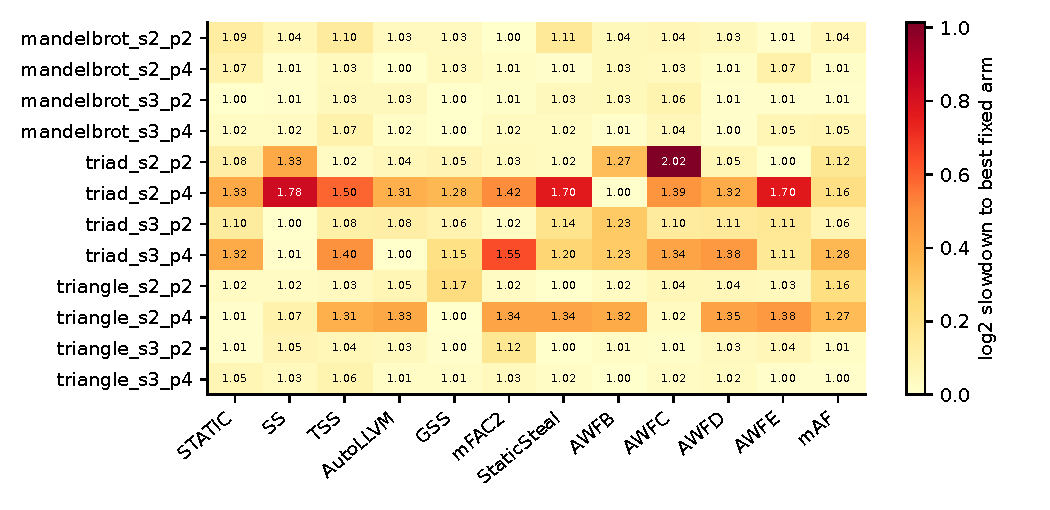
\includegraphics[width=.95\textwidth]{figures/portfolio.pdf}
\caption{Independent fixed-arm measurements on held-out scenarios.
Colors show $\log_2$ slowdown relative to the lowest median in that row;
cell labels give the untransformed runtime ratio. These are reference
measurements rather than online selector results.}
\label{fig:portfolio}
\end{figure}

\subsection{End-to-end selection cost}

\begin{table}[ht]
\centering\small
\caption{Geometric mean cumulative slowdown to the independent fixed-arm
reference. Lower values indicate less charged execution time. Prefixes
belong to the same runs; they are not separate experiments.}
\label{tab:summary}
\begin{tabular}{lrrr}
\hline
Selector & 50 instances & 144 instances & 500 instances\\
\hline
STATIC & 1.183 & 1.191 & 1.192 \\
GSS & 1.165 & 1.150 & 1.133 \\
Best fixed & 1.131 & 1.126 & 1.137 \\
Exhaustive & 1.127 & 1.141 & 1.152 \\
Native Q-learning & 1.155 & 1.169 & 1.162 \\
UCB & 1.154 & 1.156 & 1.156 \\
Cold LinUCB & 1.162 & 1.160 & 1.140 \\
Prior greedy & 1.169 & 1.163 & 1.147 \\
Warm LinUCB & 1.127 & 1.119 & 1.149 \\
Warm reduced & 1.186 & 1.172 & 1.167 \\
\hline
\end{tabular}
\end{table}

\MainResultsDiscussion{}

\begin{figure}[ht]
\centering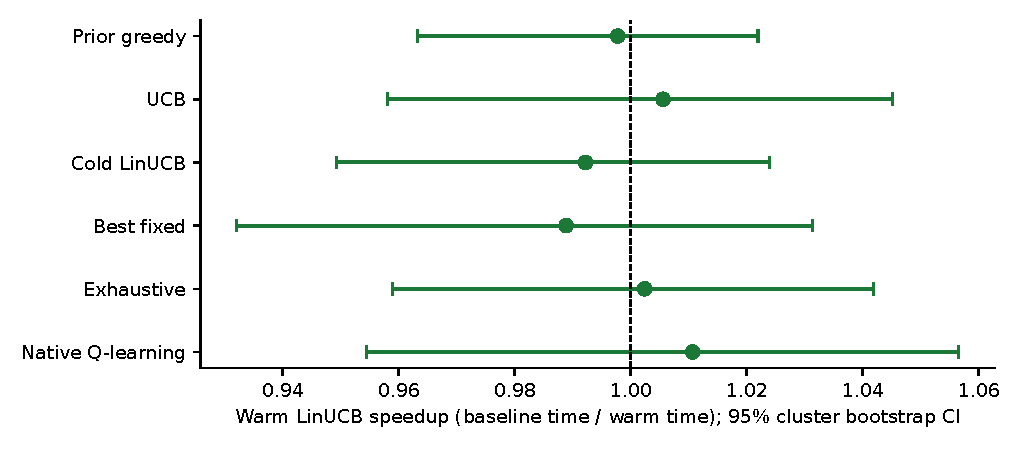
\includegraphics[width=.95\textwidth]{figures/comparisons.pdf}
\caption{Paired geometric speed ratios for full-portfolio warm LinUCB at
500 instances. Intervals use input-level cluster bootstrap resampling.
A ratio above one favors warm LinUCB; crossing one prevents a clear directional
conclusion from this interval.}
\label{fig:comparison}
\end{figure}

\subsection{Exploration and the role of the prior}

Figure~\ref{fig:trajectory} separates early execution from later behavior.
The vertical marker at instance 144 identifies the published exploration
budget, rather than guaranteeing that the released code has converged at
that instant. \ExplorationDiscussion{}

\SelectionDiscussion{}

\begin{figure}[ht]
\centering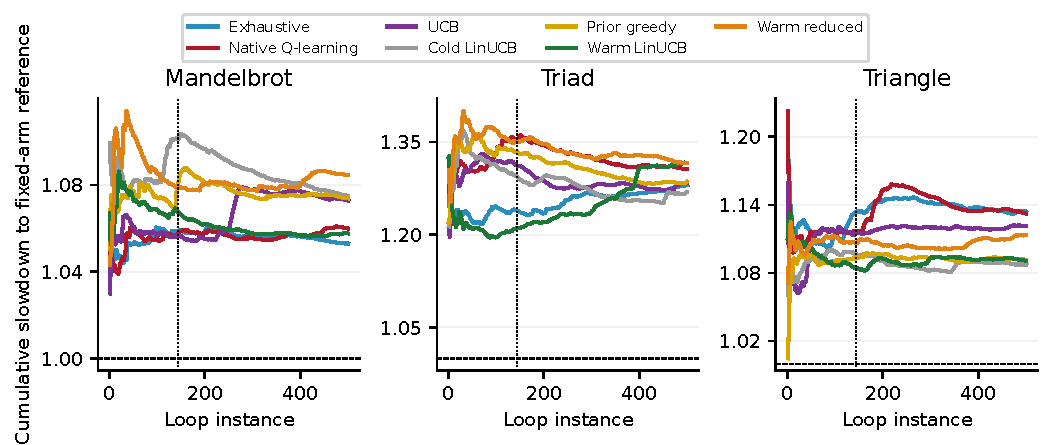
\includegraphics[width=\textwidth]{figures/trajectories.pdf}
\caption{Geometric mean cumulative slowdown on each workload family.
Each curve averages four held-out scenarios and five process repetitions.
The dashed horizontal line is the empirical fixed-arm reference. Axes are
linear; vertical scales differ between panels to show within-family behavior.}
\label{fig:trajectory}
\end{figure}

\subsection{Portfolio reduction and native overhead}

\ReductionDiscussion{}
\OverheadDiscussion{}
The median difference between full online wall-clock accounting and the sum
of charged components is \WallGap{}\%. Buffered row storage, surrounding clock
reads, and loop-control work explain this uncharged remainder; the raw
wall-clock value is retained for every run.

Excluding the interrupted fourth block gives these warm LinUCB speed ratios:
\InterruptionSensitivity{}. These are exploratory sensitivity estimates from
the remaining four blocks, not additional independent experiments.

\subsection{Exploratory transfer to an excluded workload family}

We additionally refit each prior using only the two other training workload
families, then evaluate the excluded family on its same held-out inputs.
The primary training-selected hyperparameters remain fixed. Warm LinUCB,
prior greedy, and the best fixed arm from those two families run for 500
instances in three new randomized blocks: \TransferRuns{} processes and
\TransferInstances{} additional loop instances. This experiment was added
after the primary protocol freeze and is explicitly exploratory. Its
comparisons are internal to these new blocks; it does not reuse earlier
process times as matched measurements.

\TransferDiscussion{}
Table~\ref{tab:transfer} shows the family-level breakdown. These ratios
test transfer of the fitted prior means and precision matrices. The prior weight,
regularization, and exploration coefficient were selected with calibration data
from all three families, so the
experiment is not a fully nested unseen-family hyperparameter evaluation.
With only three families and two test configurations per family, it is a
stress test rather than evidence of broad application-independent generality.
\begin{table}[ht]
\centering\small
\caption{Exploratory family-transfer speed ratios: baseline time divided by
warm LinUCB time, with each evaluated family excluded from prior fitting.
Per-family rows contain only two input configurations and are descriptive.}
\label{tab:transfer}
\begin{tabular}{lrr}
\hline
Held-out family & Versus best fixed & Versus prior greedy\\
\hline
Mandelbrot & 0.998 & 1.004 \\
Triad & 0.952 & 0.995 \\
Triangle & 1.004 & 0.990 \\
\hline
\end{tabular}
\end{table}


\section{Discussion}

The correct practical comparison is broader than replacing an expensive RL
exploration phase. If a training-selected fixed scheduler or prior-only model
already performs well, an online learner must justify both its uncertainty
trials and its update overhead. \PracticalDiscussion{}

The expected exploration advantage does not translate into an established
execution-time advantage here. Warm LinUCB concentrates on a modal arm for
most instances, yet still tries almost the full portfolio by the end of a run.
The existing expert chunk rule already controls dispatch granularity for all
methods, and several fixed-scheduler reference rows contain closely spaced
alternatives. These observations are consistent with limited incremental
value from a learned selector at this scale. They do not causally isolate
chunk sizing, core count, or workload regularity; such an attribution would
require additional controlled experiments.

The reduced portfolio also omits AWF-D, the arm selected by the training-only
best-fixed criterion. Clustering by similarity does not ensure retention of
the best aggregate arm. A future reduction rule could preserve that arm as an
additional anchor, but we retain the frozen six-arm variant in this study
rather than changing it in response to test results.

Offline training is not free. The calibration campaign executes 432 processes,
including warm-ups, graph construction, and serial correctness checks. Our
online comparison assumes those costs can be amortized across future runs.
For a single application execution, total cost must include calibration and
validation. The artifact records per-process elapsed time to make this trade-off
auditable. We do not claim a net speedup for one-off deployment that pays the
entire training campaign.

Reducing the action portfolio can limit exploration loss, but can also remove
an arm that matters on a new input. The full-portfolio ablation is therefore
essential. Similarly, the measured Q-learning result concerns one released
implementation, with its particular reward bookkeeping, initialization, and
dispatch costs. It does not imply that contextual bandits universally
outperform reinforcement learning or that the 144-round policy is the best
possible Q-learning implementation.

\section{Limitations and Threats to Validity}

\textbf{Hardware and operating environment.} One four-core WSL2 machine cannot
support claims about multi-socket HPC nodes, heterogeneous cores, NUMA effects,
or newer processors. Pinning controls guest placement but not Windows host
activity. Frequency and thermal variation may correlate across temporally
nearby runs. Randomized blocks reduce systematic treatment ordering but do not
eliminate these effects.

\textbf{Input diversity.} There are only two held-out configurations in each
workload family. Thread counts provide scaling observations but not independent
applications. Graphs are small and synthetic, and the Triad kernel may reuse
cache. The primary experiment tests transfer between related input
configurations. The exploratory family-exclusion test provides only limited
additional evidence because its hyperparameter configuration was selected
using calibration data from all three families.

\textbf{Stationarity and model assumptions.} Context is fixed after one probe.
The policy can update arm values but does not detect drift or explicitly forget
old observations. No nonstationary performance claim is supported. The linear
reward model and bounded log reward may be misspecified, particularly under
OS interruptions. STATIC imbalance and timing depend on the chunk rule;
therefore these features cannot be interpreted as intrinsic workload labels.

\textbf{Baselines and reference uncertainty.} The exhaustive selector commits
after one sample per arm and does not restart. This is a simple stationary
baseline rather than the complete Auto4OMP ExpertSel system. Cold LinUCB uses
identity initialization, so its ablation removes both fitted means and the
warm precision matrix. A single observed STATIC probe can be noisy. Reference
medians and the minimum over arms have finite-sample uncertainty; reference
slowdowns are descriptive rather than unbiased regret estimates.

\textbf{Evaluation scope.} The bootstrap has six independent input clusters;
its intervals are approximate and should not be extrapolated to an arbitrary
population of programs. Prefix horizons share observations. We do not claim
that a fixed 5\%-of-Oracle convergence target from the synopsis has been
established solely by these measurements. Larger hardware and input campaigns
are needed before making such a broad claim.

\section{Conclusion}

We implemented a complete native experiment for warm-started contextual
selection among 12 LB4OMP scheduling algorithms. Its training/test split,
serialized model, correctness checks, raw measurements, and analysis make the
comparison inspectable. \ConclusionFinding{}
The practical lesson is to evaluate an informed online selector against
exhaustive search, prior-only prediction, and a training-selected fixed policy,
and to charge every exploratory execution. The accompanying artifact provides
a concrete basis for extending this investigation to larger inputs, drift,
and additional CPU architectures.

\section*{Data, Code, and AI Assistance}

The accompanying local artifact contains source, dependency pins, build and
experiment scripts, the frozen protocol, per-process raw CSVs and manifests,
analysis code, figures, and this LaTeX source. No public repository or archival
DOI has been created; the artifact is supplied with the manuscript. An AI
coding assistant implemented the experiment and analysis, investigated
sources, and drafted this text under the authors' direction. The reported
measurements were executed in the supplied environment. The named authors
must review the scientific claims, authorship, and applicable venue disclosure
requirements before submission.

\begin{thebibliography}{99}\small
\bibitem{openmp} OpenMP Architecture Review Board.
OpenMP Application Programming Interface, Version 5.2 (2021).
\url{https://www.openmp.org/specifications/}

\bibitem{lb4omp} J.H. M\"uller Kornd\"orfer, A. Eleliemy, A. Mohammed,
and F.M. Ciorba. LB4OMP: A Dynamic Load Balancing Library for Multithreaded
Applications. IEEE TPDS 33(4), 830--841 (2022).
\url{https://doi.org/10.1109/TPDS.2021.3107775}

\bibitem{rice} J.R. Rice. The Algorithm Selection Problem.
Advances in Computers 15, 65--118 (1976).
\url{https://doi.org/10.1016/S0065-2458(08)60520-3}

\bibitem{comparative} J.H. M\"uller Kornd\"orfer, A. Mohammed, A. Eleliemy,
Q. Guilloteau, R. Krummenacher, and F.M. Ciorba. A Comparative Study of OpenMP
Scheduling Algorithm Selection Strategies. IEEE Access 13, 151216--151234
(2025). \url{https://doi.org/10.1109/ACCESS.2025.3602234}

\bibitem{auto4omp} A. Mohammed, J.H. M\"uller Kornd\"orfer, A. Eleliemy,
and F.M. Ciorba. Automated Scheduling Algorithm Selection and Chunk Parameter
Calculation in OpenMP. IEEE TPDS 33(12), 4383--4394 (2022).
\url{https://doi.org/10.1109/TPDS.2022.3189270}

\bibitem{auer} P. Auer, N. Cesa-Bianchi, and P. Fischer.
Finite-time Analysis of the Multiarmed Bandit Problem. Machine Learning 47,
235--256 (2002). \url{https://doi.org/10.1023/A:1013689704352}

\bibitem{linucb} L. Li, W. Chu, J. Langford, and R.E. Schapire.
A Contextual-Bandit Approach to Personalized News Article Recommendation.
In WWW, 661--670 (2010). \url{https://doi.org/10.1145/1772690.1772758}

\bibitem{oetomo} B. Oetomo, R.M. Perera, R. Borovica-Gajic, and
B.I.P. Rubinstein. Cutting to the Chase with Warm-Start Contextual Bandits.
Knowledge and Information Systems 65, 3533--3565 (2023).
\url{https://doi.org/10.1007/s10115-023-01861-2}

\bibitem{stream} J.D. McCalpin. STREAM: Sustainable Memory Bandwidth
in High Performance Computers. \url{https://www.cs.virginia.edu/stream/}

\bibitem{gap} S. Beamer, K. Asanovi\'c, and D. Patterson.
The GAP Benchmark Suite. arXiv:1508.03619 (2015).
\url{https://arxiv.org/abs/1508.03619}

\bibitem{kalibera} T. Kalibera and R. Jones.
Rigorous Benchmarking in Reasonable Time. In ISMM, 63--74 (2013).
\url{https://kar.kent.ac.uk/33611/}
\end{thebibliography}
\end{document}
